\documentclass{article}
\usepackage{amssymb}
\usepackage[dutch]{babel}
\usepackage{a4wide}
\usepackage{graphicx}
\newcommand{\cat}{+\!\!\!\!+\:}
\newcommand{\inr}{< \!\!\!\!\!\! - \:}

\title{Procesdocument OGO 1.1}
\author{Edin Dudojevic, Leroy Bakker}

\DeclareGraphicsRule{.tif}{png}{.jpg}{`convert #1 `dirname #1`/`basename #1 .tif`.png}

\begin{document}

\maketitle

\section{Project 1}
\subsection{Tijdverdeling}
% Hoeveel tijd er door de verschillende groepsleden is besteed aan het project.
 Iedereen heeft zijn eigen logboek op een online
systeem bijgehouden op lms.ogotue.nl.
\newline
(Zie bijlage voor een gedetailleerd overzicht van het logboek)
\subsubsection{Voorzitter, Notulist} De voorzitter en notulist werden
per week omgewisseld. De vergadering werd gehouden op elke woensdag
die een tijdsduur had van een half uur.
\newline

\begin{tabular}{c l l l}
  \hline
  % after \\: \hline or \cline{col1-col2} \cline{col3-col4} ...
  Id-nummer & Naam & Notulist & Voorzitter\\
  \hline
  0617167 & Leroy Bakker & Week 36 & Week 37 \\
  0608170 & Roy Berkeveld & Week 37 & Week 38 \\
  0615787 & Giso Dal & Week 38 & Week 39 \\
  0618959 & Etienne van Delden & Week 39 & Week 40 \\
  0608206 & Edin Dudojevic & Week 40 & Week 41 \\
  0587266 & Nick van der Veeken & Week 41 & Week 36 \\

  \hline
\end{tabular} \\

\subsection{Taakverdeling}
% Hoe de taken zijn verdeeld

\subsubsection{Voorzitter, Notulist}

De rollen van voorzitter en notulist zijn per week omgewisseld en zo
is iedereen een keer aan de beurt geweest. Omdat de taak verdelening goed 
verlopen is en iedereen tevreden is met de huidige aanpak ervan,
blijven we de routine gebruiken bij het tweede deel van het project.

\subsubsection{Opgaven}

De opgaven zijn in de eerste week gezamenlijk behandeld en nagekeken. De weken erna is de groep opgesplit in een
'maak-groep' en een 'controle-groep'. De maak-groep heeft individueel de gegeven opdrachten gemaakt en de controle-groep
vervolgens de resultaten gecontroleerd en een verslag gemaakt in een peer-review.
\newline

De rij van de oplossingen is bijgehouden en verspreid van de recentste versies onder de leden door Roy Berkeveld.
\newpage
\subsubsection{Productdocument}
Het productdocument is gecoordineerd en opgezet door Etienne van
Delden. Dit was pas mogelijk nadat alle opgaven waren gemaakt en
 door de leden gezamenlijk gecontroleerd. Dit was een week voor de harde deadline ingeleverd bij Martijn zodat we mogelijke fouten voor de echte
deadline konden verbeteren.

Er werden een bepaald aantal fouten aangewezen in het productdocument door Martijn die nodig opnieuw bekeken moesten worden. In
de vierde en vijfde week is vervolgens alles op orde gezet.

\subsubsection{Procesdocument}
Het procesdocument is opgemaakt met als basis de eerder gemaakte
notulen. Alles omtrent het verloop van het project is hier opgesomd
en beschreven. Het procesdocument is gemaakt door Edin Dudojevic.


\subsection{Peer reviews}
De peer reviews zijn opgenomen in het productdocument samen met de
opgaven. Bij elke opgave waarbij iets op te merken was werd een peer
review gegeven. Indien het nodig was werd de opgave gezamenlijk
gecontroleerd op fouten en opnieuw gemaakt.�

\subsection{Peer assessments}
De in te vullen peer assessments zijn in week 5 door Martijn aan de
leden van de groep uitgedeeld. Ieder lid heeft een ander lid
beoordeeld door middel van een beoordelingstabel. De uitkomst
hieruit is weergegeven in figuur \ref{fig:pac1}. De hoogst te
behalen score is 25.

\begin{figure}[h] % figure placement: here, top, bottom, or page
\centering
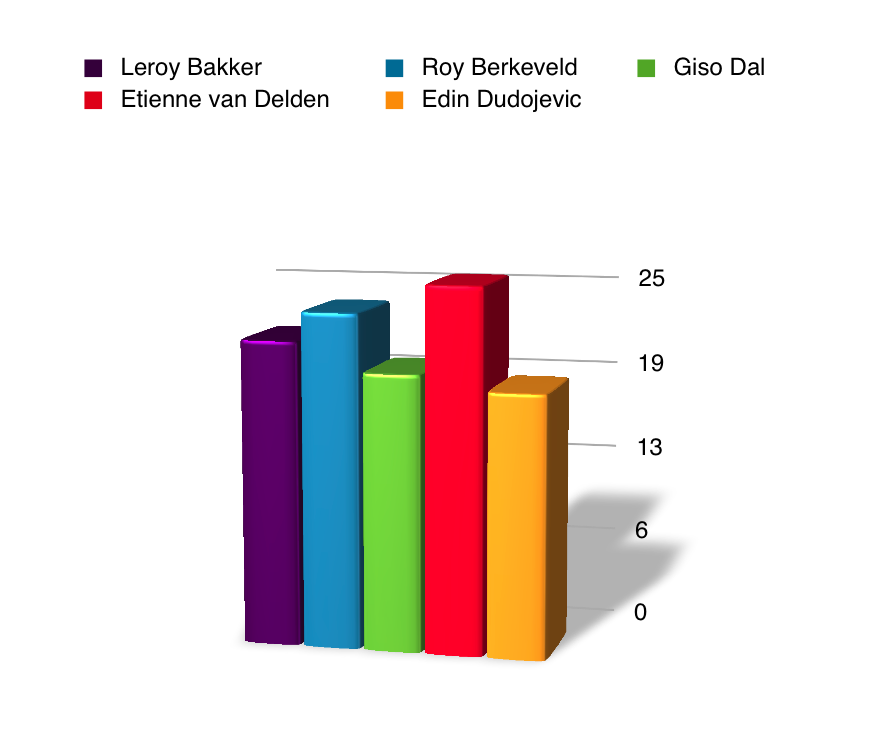
\includegraphics[width=4in]{peerassesmentchart.png}
\caption{Peer Assessment Chart 1} \label{fig:pac1}
\end{figure}
\newpage

\subsection{Evaluatie van het project}
%Terugblik op de opdracht met goede en minder goede punten daarin

\subsubsection{Dubbelzinnigheid}
Er waren meerdere opgaven die konden leiden tot verschillende
interpertaties. Dit heeft er wel toe geleid dat wij na verloop van
tijd steeds kritischer de opdrachten gingen benaderen om zo
mogelijke specificatiefouten te voorkomen.

Het was zowel een kunst als een uitdaging om van een bepaalde specificatie geen beschrijving maar een heldere en duidelijke formulering van te maken.

\subsubsection{Specificatie}
Wat ook duidelijk opviel waren de verschillen tussen de specificatie
in mathematische en de Nederlandse taal. Omdat de wiskunde zo veel
preciezer is om iets uit te drukken dan de gewone taal, was
duidelijk te merken dat er bij de omzetting naar het Nederlands veel
meer ``taal'' gebruikt moest worden om alles zo precies mogelijk, maar
toch niet al te letterlijk te formuleren. Het moest aan de eisen
voldoen': 'Kort maar krachtig'.


\subsection{Conclusie}
Na vier weken werken aan dit eerste OGO project ligt er een
productverslag op tafel dat in $\LaTeX$ is gemaakt. In de eerste
week is er kennisgemaakt binnen de groep en is er een planning
gemaakt voor het verdere verloop van het project. Oefening met
$\LaTeX$ was vereist om gemaakte opgaven op een praktische manier in
een digitaal document om te zetten.

Na de derde bijeenkomst was voor iedereen het hoe en wat van OGO duidelijk. Vergaderingen werden geleid door een voorzitter,
genotuleerd door een notulist en bijgewoond door alle groepsleden en een tutor. Ook de opgedane kennis over $\LaTeX$ kon na twee
weken in de praktijk worden gebruikt voor het invoeren van mathematische formules.

Na het maken en controleren van de opgaven is een document gemaakt met daarin de antwoorden van alle opgaven bij elkaar. In de
voorlaatste week is dit document uitgebreid met onder andere een samenvatting, conclusie en een literatuurlijst.

\newpage

\section{Project 2}

\subsection{Tijdverdeling}
% Hoeveel tijd er door de verschillende groepsleden is besteed aan het project.
 Het logboeksysteem is gewijzigd tijdens project 2. Wij zijn
 overgestapt van het online logboeksyteem lms.ogotue.nl naar een
\TeX-bestand op onze SVN-server. Hierdoor bestaat de bijlage uit
 twee verschillende versies van het logboek.
\newline
(Zie bijlage voor een gedetailleerd overzicht van het logboek)

\subsubsection{Voorzitter, Notulist} De voorzitter en notulist werden
per week omgewisseld. De vergadering werd gehouden op elke woensdag
die een tijdsduur had van een half uur.
\newline
Door het uitvallen van Nick van der Veeken bij project 2 is er het
een en ander aan de routine veranderd.
\newline

\begin{tabular}{c l l l}
  \hline
  % after \\: \hline or \cline{col1-col2} \cline{col3-col4} ...
  Id-nummer & Naam & Notulist & Voorzitter\\
  \hline
  0617167 & Leroy Bakker & Week 43 & Week 44 \\
  0608170 & Roy Berkeveld & Week 44 & Week 45 \\
  0615787 & Giso Dal & Week 45 & Week 46 \\
  0618959 & Etienne van Delden & Week 46 & Week 42 \\
  0608206 & Edin Dudojevic & Week 42 & Week 43 \\

  \hline
\end{tabular}

\subsection{Taakverdeling}
% Hoe de taken zijn verdeeld

\subsubsection{Voorzitter, Notulist}

De bedoeling was dat we de routine van project 1 zouden behouden,
maar door het plotselinge uitvallen van Nick van der Veeken kon dat
helaas niet en moest er een kleine aanpassing in de taakverdeling
worden gemaakt.

\subsubsection{Opgaven}

Omdat productdocument 1 werd afgekeurd, moest deze eerst worden
verbeterd. Bovendien hebben we 30 extra oefenopgaven gekregen, die
project 2 vormden.
\newline

Voor het verbeteren van productdocument 1 hebben we de groep
onderverdeeld in drie groepjes van twee personen. Ieder groepje
kreeg een aantal opgaven toegewezen en maakte deze. De gemaakte
opgaven werden via de SVN-server bijgehouden en vervolgens door de
twee andere groepjes nagekeken en zonodig verbeterd.
\newline

De 30 extra oefenopgaven hebben we individueel verdeeld. Ieder kreeg
5 opgaven toegewezen. De gemaakte opgaven werden vervolgens door
drie andere personen nagekeken. Hiervoor hebben we een speciaal
\TeX-bestand bijgehouden waarin iedereen zijn peer review kon
toevoegen. Met behulp van deze peer reviews werden de afgekeurde
opgaven verbeterd.

\newpage
\subsubsection{Productdocument}
Productdocument 2 is gecoordineerd en opgezet op onze SVN-server.
Omdat er voor de opgaven templates waren gemaakt, waren deze
gemakkelijk toe te voegen en te updaten. De rest van productdocument
2 werd gemaakt door Giso Dal.
\newline

Er werden door Martijn in de voorlopige versie van productdocument 2
een aantal opgaven aangewezen die opnieuw bekeken en verbeterd
moesten worden. Dit is in de laatste week van project 2 verbeterd.

\subsubsection{Procesdocument}
Het procesdocument is opgemaakt met als basis de eerder gemaakte
notulen. Alles omtrent het verloop van het project is hier opgesomd
en beschreven. Het procesdocument is gemaakt door Edin Dudojevic
(project 1) en Leroy Bakker (project 2).

\subsection{Peer reviews}
De peer reviews zijn opgenomen in het productdocument samen met de
opgaven. Deze peer reviews stonden op onze SVN-server bij iedere
opgave. Indien in de peer review werd vermeld dat de opgave onjuist
was, werd de opgave gezamenlijk gecontroleerd en indien nodig
opnieuw gemaakt.

\subsection{Peer assessments}
De in te vullen peer assessments zijn door Martijn aan de leden van
de groep uitgedeeld. Ieder lid heeft een ander lid beoordeeld door
middel van een beoordelingstabel. De uitkomst hieruit is weergegeven
in figuur \ref{fig:pac2}. De hoogst te behalen score is 20.

\begin{figure}[h] % figure placement: here, top, bottom, or page
\centering
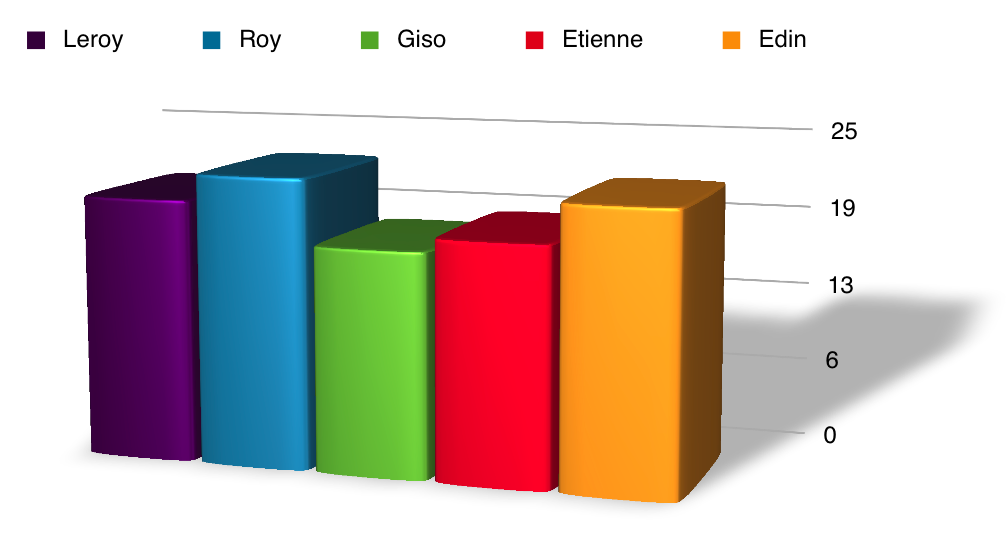
\includegraphics[width=4in]{peerassesmentchart2.png}
\caption{Peer Assessment Chart 2} \label{fig:pac2}
\end{figure}
\newpage

\subsection{Evaluatie van het project}
%Terugblik op de opdracht met goede en minder goede punten daarin

\subsubsection{Dubbelzinnigheid}
Ook nu weer waren er opgaven die konden leiden tot verschillende
interpertaties. Maar dit werd onderling goed opgelost door
argumentatie of door een aanname aan de opdracht toe te voegen.

\subsubsection{Specificatie}
Wat opviel was dat project 2 toch iets soepeler verliep met
specificeren en reviewen. Omdat bij project 1 nog alles moest worden
doorgenomen en nu alles al was behandeld, ging het maken van de
opdrachten sneller. Ook het onderling overtuigen van goede of
foutieve opgaven ging een stuk makkelijker omdat de kennis nu groter
was dan bij project 1.


\subsection{Conclusie}
Na het afronden van project 2 was duidelijk zichtbaar dat we
vooruitgang hebben geboekt wat betreft specificeren. Project 2
verliep veel soepeler dan project 1 omdat de kennis over logica en
verzamelingleer is uitgebreid.

Het was jammer dat Nick van der Veeken stopte met OGO 1.1. We merkte
dat met een mankracht minder, meer werk te doen was.

Het invoeren van de SVN-server gaf veel meer structuur in onze
manier van werken. Iedereen kon nu individueel aan de opdrachten
werken en reviewen. Iedereen kon opdrachten en verbeteringen
toevoegen en deze van andere bekijken. Deze manier van werken zorgde
ervoor dat er veel gemakkelijker kon worden gereviewd.

Na het maken en controleren van de opgaven is productdocument 2
gemaakt met daarin de antwoorden van alle opgaven bij elkaar. De
extra opgaven hebben er zeker voor gezorgd dat ons specificeren is
verbeterd.

\newpage

\section{Bijlage}

\subsection{Logboek}

\subsection{Notulen}

\end{document}
